\documentclass[a4paper,12pt]{article}
\usepackage{fullpage}
\usepackage[T1]{fontenc}
\usepackage{amsmath}
\usepackage{amssymb}
\usepackage[utf8]{inputenc}
\usepackage{color}
\usepackage{authblk}
\usepackage{todonotes}
\usepackage{caption}
\usepackage{url}
\usepackage{float}
\usepackage{sectsty}
\usepackage{pdfpages}
\usepackage[section]{placeins}
\DeclareCaptionFont{white}{\color{white}}
\DeclareCaptionFormat{listing}{\colorbox{gray}{\parbox{\textwidth}{#1#2#3}}}
\captionsetup[lstlisting]{format=listing,labelfont=white,textfont=white}

\usepackage{setspace}
\usepackage[toc,page]{appendix}
\usepackage{framed}
\usepackage{geometry}

\usepackage{alltt}
\usepackage{subfig}

% Change section fonts
\allsectionsfont{\sffamily}

% For code box
\usepackage{xcolor}
\usepackage{listings}
\usepackage{caption}
\DeclareCaptionFont{white}{\color{white}}
\DeclareCaptionFormat{listing}{%
  \parbox{\textwidth}{\colorbox{gray}{\parbox{\textwidth}{#1#2#3}}\vskip-4pt}}
  \captionsetup[lstlisting]{format=listing,labelfont=white,textfont=white}
  \lstset{frame=lrb,xleftmargin=\fboxsep,xrightmargin=-\fboxsep}
% End code box

\usepackage{cite}

% General parameters, for ALL pages:
\renewcommand{\topfraction}{0.9}	% max fraction of floats at top
\renewcommand{\bottomfraction}{0.8}	% max fraction of floats at bottom
% Parameters for TEXT pages (not float pages):
\setcounter{topnumber}{2}
\setcounter{bottomnumber}{2}
\setcounter{totalnumber}{4} % 2 may work better
\setcounter{dbltopnumber}{2} % for 2-column pages

\addtolength{\topmargin}{0.5in}

\usepackage{fancyvrb}

\usepackage{tikz} \usetikzlibrary{trees}
\usepackage{hyperref} % should always be the last package

% useful colours (use sparingly!):
\newcommand{\blue}[1]{{\color{blue}#1}}
\newcommand{\green}[1]{{\color{green}#1}}
\newcommand{\red}[1]{{\color{red}#1}}

% useful wrappers for algorithmic/Python notation:
\newcommand{\length}[1]{\text{len}(#1)}
\newcommand{\twodots}{\mathinner{\ldotp\ldotp}} % taken from clrscode3e.sty
\newcommand{\Oh}[1]{\mathcal{O}\left(#1\right)}

% useful (wrappers for) math symbols:
\newcommand{\Cardinality}[1]{\left\lvert#1\right\rvert}
\newcommand{\Ceiling}[1]{\left\lceil#1\right\rceil}
\newcommand{\Floor}[1]{\left\lfloor#1\right\rfloor}
\newcommand{\Iff}{\Leftrightarrow}
\newcommand{\Implies}{\Rightarrow}
\newcommand{\Intersect}{\cap}
\newcommand{\Sequence}[1]{\left[#1\right]}
\newcommand{\Set}[1]{\left\{#1\right\}}
\newcommand{\SetComp}[2]{\Set{#1\SuchThat#2}}
\newcommand{\SuchThat}{\mid}
\newcommand{\Tuple}[1]{\langle#1\rangle}
\newcommand{\Union}{\cup}
\usetikzlibrary{positioning,shapes,shadows,arrows}
\providecommand{\keywords}[1]{\textbf{\textit{Keywords: }} #1}

\title{\textbf{Providing an Access Control Layer for Content Distribution Networks}}
\author{Lukas Klingsbo}

\begin{document}

\maketitle
%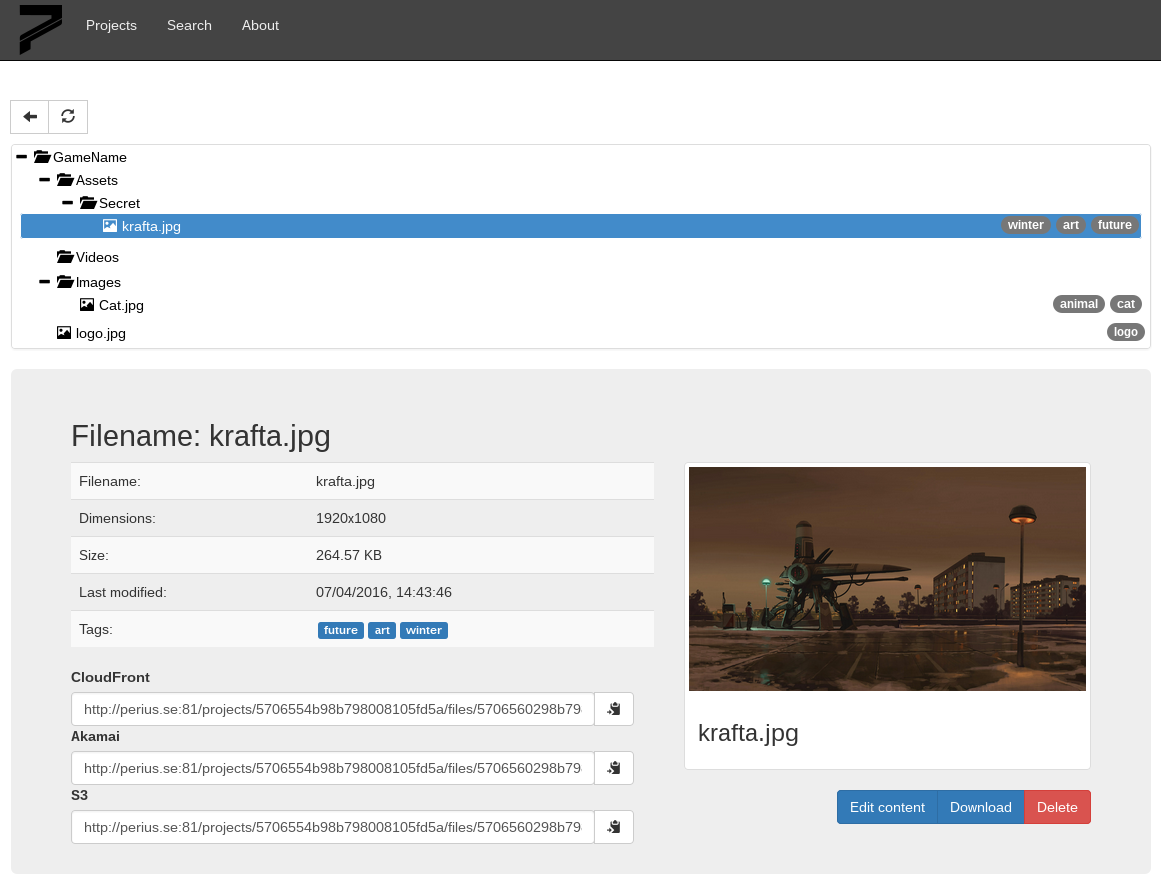
\includepdf[pages={1}]{front.pdf}
%\thispagestyle{empty}
%\newpage\null\thispagestyle{empty}\newpage

\pagenumbering{roman}
\setcounter{page}{2}

%\includepdf[pages={1}]{abstract.pdf}
\begin{abstract}
    TODO: Abstract

\keywords{}
\end{abstract}

\newpage\null\thispagestyle{empty}\newpage

\setcounter{tocdepth}{3}
\tableofcontents

\clearpage
\pagenumbering{arabic}
\setcounter{page}{1}
\section{Introduction}
Developing larger projects containing static content usually involves using a Content Distribution Network 
to be able to scale to a large user base. The commercial Content Distribution Networks are usually fairly easy to use, 
the content that is to be used in a project is usually simply uploaded and then directly available to the public. 
For secret content this can be a problem and that is what this thesis is about. This work examines ways of enforcing 
access control on content and groups of content in the form of views. A system was developed to make the underlying 
theory work in practice. 

\newpage
\section{Related Terminology}
\subsection{Technologies}
\subsubsection{React}
React is a JavaScript library for building user interfaces. React uses both its own virtual DOM and the browser's, 
this makes it able to efficiently update dynamic web pages after a change of state through comparing the old virtual 
DOM with the resulting virtual DOM after the state change and then only update the browser's DOM according to the 
difference between the virtual DOMs~\cite{REACT}.

\subsubsection{Flux}


\subsubsection{Scala}
Scala is a multi-paradigm programming language. It most commonly runs on the JVM and compared to Java it supports 
most functional programming features at the same time as it supports object oriented programming~\cite{SCALA}.

\subsubsection{JSON-RPC}
Over http? WebSockets? 
\subsubsection{TODO: Insert persistent storage here}
    TODO: Write down related terminology, if any
\subsection{Abbreviations}

\subsubsection{CDN}
Content Distribution Network - Replicates content to several servers, usually spread out geographically. Once a 
request is made, the network serves content from the server closest to the requester.

\section{Background}
\subsection{About Uprise}
Uprise is a company based in Uppsala, Sweden. 

\subsection{The current system}
Maybe write about battlebinary?  

\subsection{Problem description}
Having
  
Battle Binary

What is needed
* Security layers
* Views
* Virtual file structure
* Versioning of content
* Multi project support
* Auth and audit logs
* Users

\section{Methods for determining\\implementation details}
This chapter introduces the different methods used to determine how the new system should be implemented, which DBMS it should use and how the estimation of long term scaling was done.

\section{Security of the system}
\subsection{Authorization}
\subsection{Audit logs}


\section{Resulting system}
\subsection{Scalability}

\section{Discussion}

\section{Summary}
\subsection{Conclusions}

\subsection{Future work}

Stuff to write about:
Modular design, every piece should be interchangable
LDAP - why it was used as standard AUTH


\newpage
\bibliographystyle{ieeetr}
\bibliography{references}

\end{document}
